\section{Motivation, innovation, and specific aims}

\subsection{Motivation}
    The basis of this proposal is fulfilling the lack of knowledge on the underlying mechanism driving the fatigue and failure of BHV devices, which is the major hurdle impede the development on new BHV technologies. Traditionally, the development of BHV starts with simple mechanical characterization for their ability to handle their mechanical demands, and accelerated wear testing (AWT) at 10-15 time normal physiological rate to evaluate durability. Successful designs are then put through animal models and clinical testing. The first stage offers only simple understanding of the functional properties and durability of these devices while the latter is a complex and unpredictable system and the ultimate cause of failure is difficult to be understood. Thus the crux of this proposal is the lack of a more rigorous approach that better utilities in vitro experimental measurements and fundamental understanding of structure-functional relationship to predict the performance of BHVs.

\subsection{Innovations}
\subsubsection{The Lack of Established Constitutive Models for Planar Soft Tissues}
    Although finite element analysis is an effective method for stress analysis, truly predictable computational simulations cannot be done without an accurate constitutative model for the underlying biomechanical response. There is currently a lack of a well establish constitutive model for collagenous soft tissues. Currently each research group uses their own model, often simple forms of the Fung model or linear functions of the invariants. These models are often not informative, offering no insights into the structural functional relationship. Unfortunately, this also means these models are also lack predictive capabilities as a result, and can only interpolated the experimental data. This is a problem for simulating the effect of fatigue in which the geometry and the mechanical properties of BHVs can change significantly, necessating extrapolation of the data into unmeasured regime. Structural models theories exists \cite{sacks_incorporation_2003,lanir_structural_1979,driessen_structural_2005} but is under utilized and not well validated for the wide range of tissue that may be applicable for BHV devices. Thus, the establishment of a generalized and well-validated constitutive model is a critical step the in process of developing accurate simulations of BHV devices.

\subsubsection{The Lack of Fundamental Modeling Approach for EXLs, PS, and Collagen Fiber-Level Damage in Soft Tissue-Derived Biomaterials}

    There is no accepted constitutive model for the effect of EXLs on the mechanical properties of soft tissues. Without understanding the mechanical properties of the subcomponents of the bioprosthetic biomaterial, we cannot properly predict how they will change over time. Although calcification plays an important role in the failure of BHVs, addressing this concern alone will not alleviate the loss of functional due to mechanical fatigue. Although this proposal will not simulate the full process to failure, as previously indicated (1.B), we will for the first time examine the early stages of fatigue in PS and collagen fiber-level damage. This will nevertheless give us a firsthand estimate of BHV durability and design, as well as build the foundation for future extensions of the model.

\subsubsection{The Lack of A Framework for Simulating The Response of BHV Devices in Response to Cyclic Loading}

    Our ability to evaluate the design of BHVs devices are directly linked to our ability to understand and rigorously experiment on the in vivo durability of these devices. However, clinical and large anime testing remains costly and reserved for latter stages of the design analysis. Furthermore, it is difficult for such studies to paint a complete picture of the underlying mechanisms due bio-variability and direct ways of controlling the biological system. This has led to a stagnation of BHV device development \cite{schoen_cardiac_2005}. Computational simulations can be an exceptional complement to in vitro and animal experiment in understanding how biomechanical properties evolve and drive mechanical function and performance. Indeed, the consensus in the field is the increasing role of computational simulation in the development of cardiovascular devices. Finite element analysis is unknown for its ability to determine the stress at a device-level and can be used to reiterate on conceptual designs to optimize the functional properties of prototypes \cite{patterson_comparative_1996,huang_two_1990,black_three_1991}. Thus, computational implementation of the tissue structural PS-fatigue model is the best way to guide our understanding of BHV device performance.

\subsection{Specific aims}
    Soft-tissue-derived exogenously cross-linked (EXL) biomaterials continue to play an important role in surgical repair and medical devices. This is especially true for bioprosthetic heart valves (BHV), by having advantages in immunogenic and mechanical behaviors \cite{starr_artificial_2007}. Despite ongoing research, our understanding of these materials and of the mechanisms leading to their failure remains at an empirical level. The need for advancements in predicting the material behavior is further underscored by the development of percutaneously-delivered BHV devices. While these devices reduce surgical risk, they also present additional challenges for the design of the BHVs due to limitations in thickness, and folding and compression during delivery. A significant challenge prohibiting accurate and predictive simulations of BHVs are a lack of understanding of the effect of exogenous cross-linkers, such as glutaraldehyde (GLUT), and an associated predictive material model in response to cyclic loading. GLUT EXLs form polymeric chains through the cross-linking process which more tightly bond the collagen fibers to the non-fibrous matrix, increasing the non-fibrous matrix stiffness and fiber-fiber interactions. However, GLUT EXLs also undergo Schiff-base reactions that are hypothesized to lead to scission-healing behaviors that result in the permanent set (PS) phenomena. PS continuously changes in the reference geometry of the BHV and can induce extra-physiological stress concentrations in the BHV leaflets. Microstructural-based constitutive models for tissues and their use in valve-level simulations can lead to insights into the underlying mechanisms and more accurate prediction of their long-term performance. Thus, we seek to develop a framework for modeling and simulating biologically-derived EXL soft collagenous tissues for BHV, accounting for the effects of EXL, PS, and collagen fiber-level damage, taking the following approach:


    \subsubsection*{Specific Aim 1: Establish and validate a generalized nonlinear hyperelastic meso-scale structural constitutive model (MSSCM) for native collagenous soft tissues.} As a first step towards modeling EXL biomaterials, we will take a generalized meso-scale (at the level of the constituent fibers) structural modeling approach to accurately model the mechanical response of soft tissues. Firstly, we will develop an improved analytical method for processing extant mechanical data under generalized 2D deformations, to more accurately characterize the tissue. Next, after posing the model form, we will extensively validate critical assumptions such as affine fiber deformation, mechanical response of the constituent fibers, and direct integration of physical measurements of the fiber microstructure. The validation will be done through extensive mechanical characterization through different testing methods and microstructural characterization at the 1) micro-scale (fibril) and 2) meso-scale using optical techniques such as multiphoton microscopy and x-ray scattering. The two tissues we will examine for application and validation of the model are the ovine pulmonary artery and the porcine mitral valve leaflets, which offer a diverse selection structural composition to span applicable realms.
    
    \addcontentsline{toc}{subsubsection}{Specific Aim 1: Establish and validate a generalized nonlinear hyperelastic meso-scale structural constitutive model for native collagenous soft tissues.}%


    \subsubsection*{Specific Aim 2: Extend the MSSCM to account for of the presence of EXLs and subsequent response to continuous cyclic loading.} Using GLUT treated bovine pericardium, we aim to separately model the mechanical response of the collagen fibers, matrix, and fiber-fiber interactions due to cross-linking. For this, we will develop a method to map the collagen fiber architecture characterized from the native state to the EXL state. Next, we will develop a PS model based on a constantly evolving referential configuration that occurs due to scission-healing when the tissue is held in an extended state. We will validate the model for orientation and strain level dependence. The model will be tested and validated using constant cyclic strain, as well as stress control experimental data. Finally, we will extend the model for collagen fiber-level damage that may occur during cyclic loading. 
    
    \addcontentsline{toc}{subsubsection}{Specific Aim 2: Extend the meso-scale structural constitutive model to account for of the presence of EXLs and subsequent response to continuous cyclic loading.}%
    
    
    \subsubsection*{Specific Aim 3: Application to organ/device level.} In this final aim, we will develop a full 3D finite element framework for the simulation of permanent set utilizing an effective model approach, acting as an intermediate between the predictive constitutive model and the numerical implementation. This approach has great potential to improve the computational efficiency of numerical simulations using multi-scale or structural modeling approaches. We will parametrically explore initial geometries and material properties which may minimize the risks of these effects. With this, we aim to develop a better understanding of the underlying process that occurs during long-term cyclic loading using our constitutive modeling approach and device level applications, and translate the insights gained to improving BHV design and durability. 

    \addcontentsline{toc}{subsubsection}{Specific Aim 3: Application to organ/device level}%
    
    
%-------------------	begin FIGURE 	-------------------%
\begin{figure}
\centering
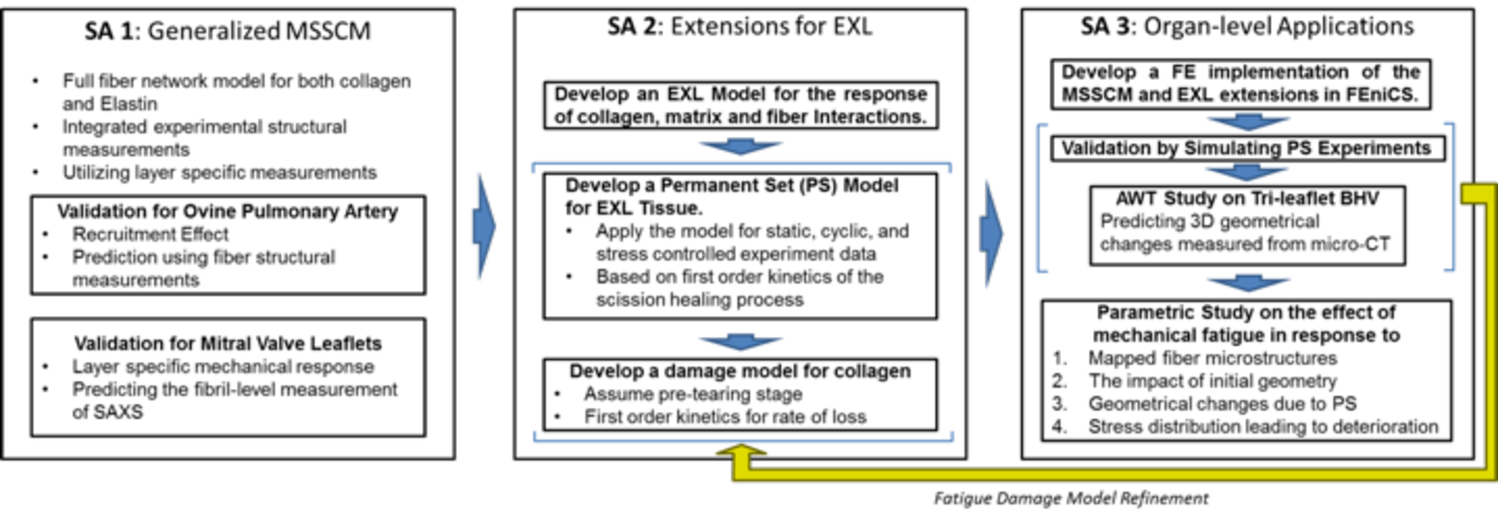
\includegraphics[width=\textwidth]{Images/chapter1/specificaims.pdf}
\caption{Overview of the entire project, showing how we will develop a FDM model for a BHV starting from with a generalized model of its mechanical response (SA 1) and extended for cross-linking effects including the stiffening of the matrix, increasing of collagen fiber-fiber interactions and PS (SA 2) and finally applied at the organ-level using a finite element framework (SA  3).}
\label{c1:fig:specificaims}
\end{figure}
%-------------------	 end FIGURE 	-------------------%